\appendix

\chapter{Survey} \label{survey}
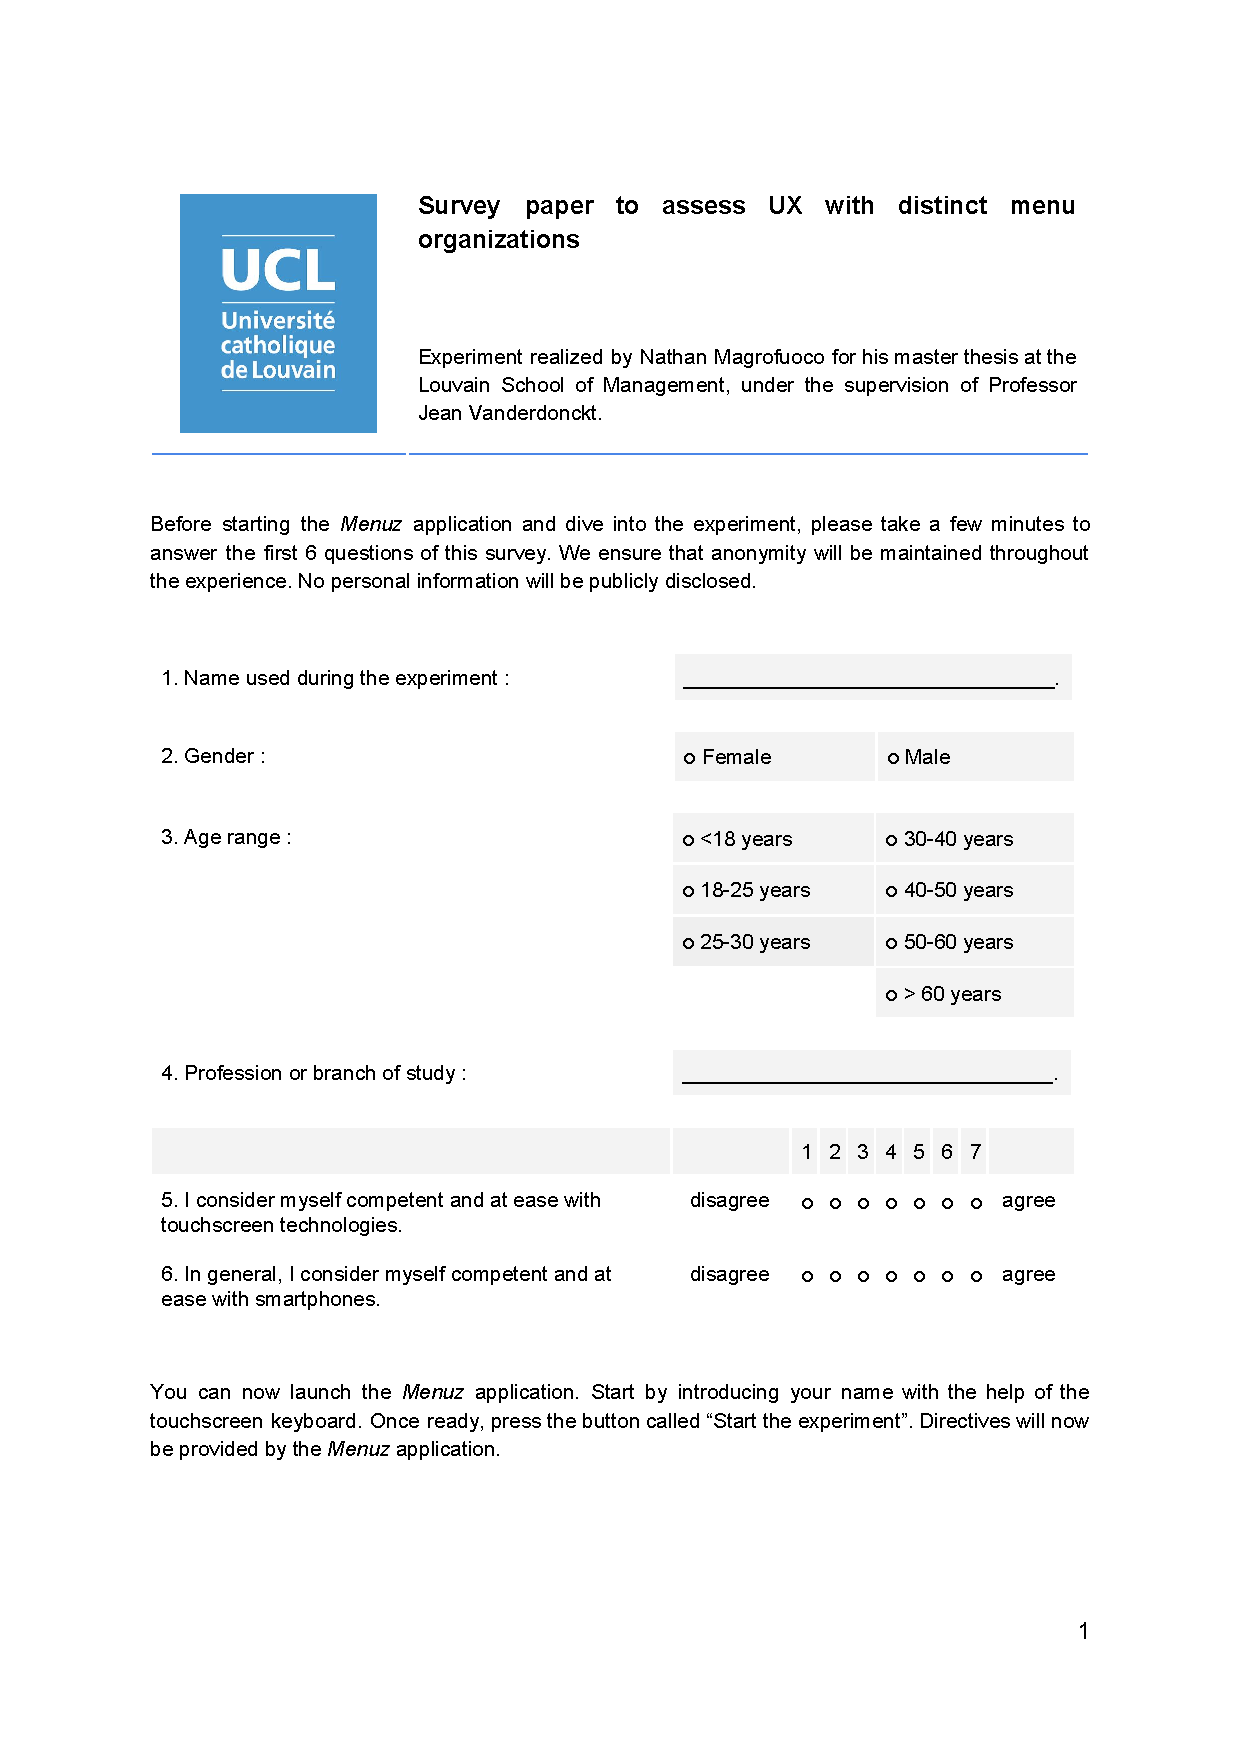
\includepdf[pages={1-},scale=0.85]{img/survey.pdf}

\chapter{Application UI} \label{screenshots}

\newpage

\begin{figure}[!ht]
  \begin{center}
    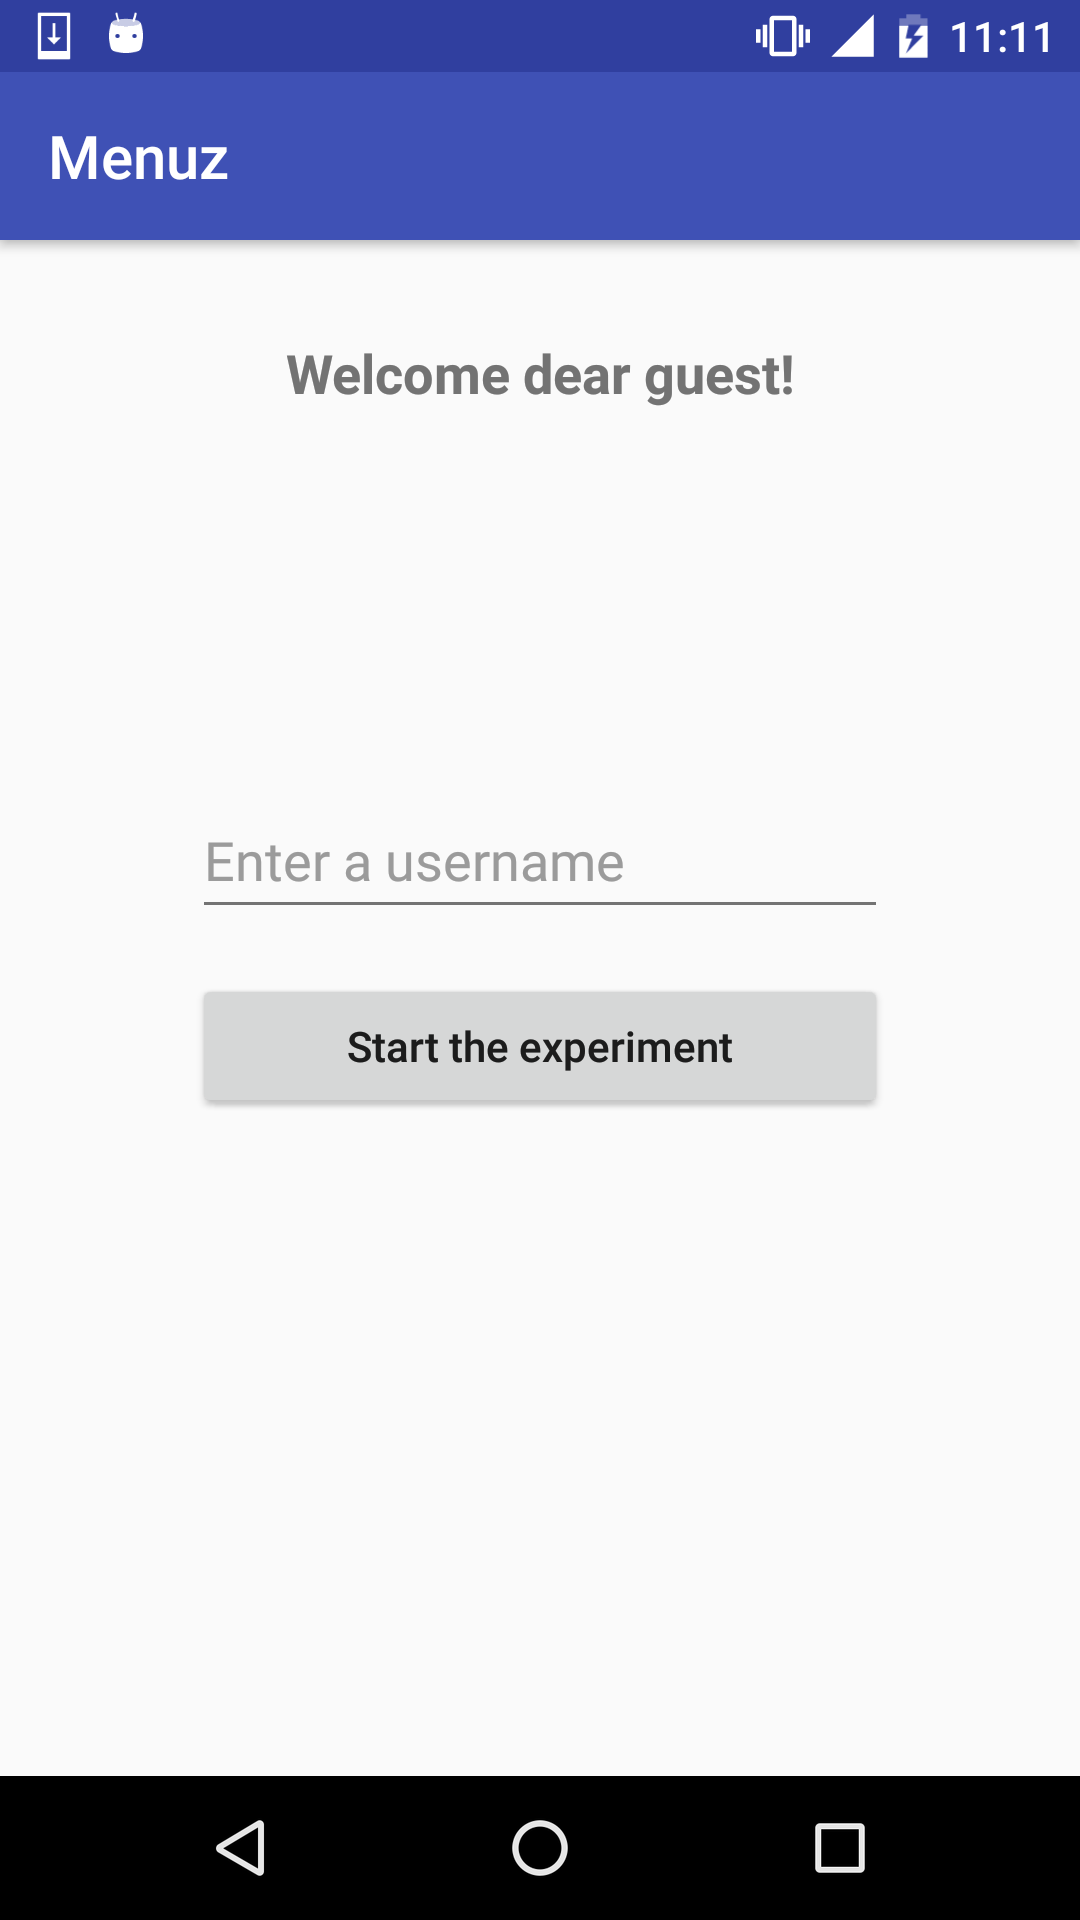
\includegraphics[scale=0.22]{img/main_activity.png}
    \label{fig:main_activity}
    \caption{MainActivity.}
  \end{center}
\end{figure}

\newpage

\begin{figure}[!ht]
  \begin{center}
    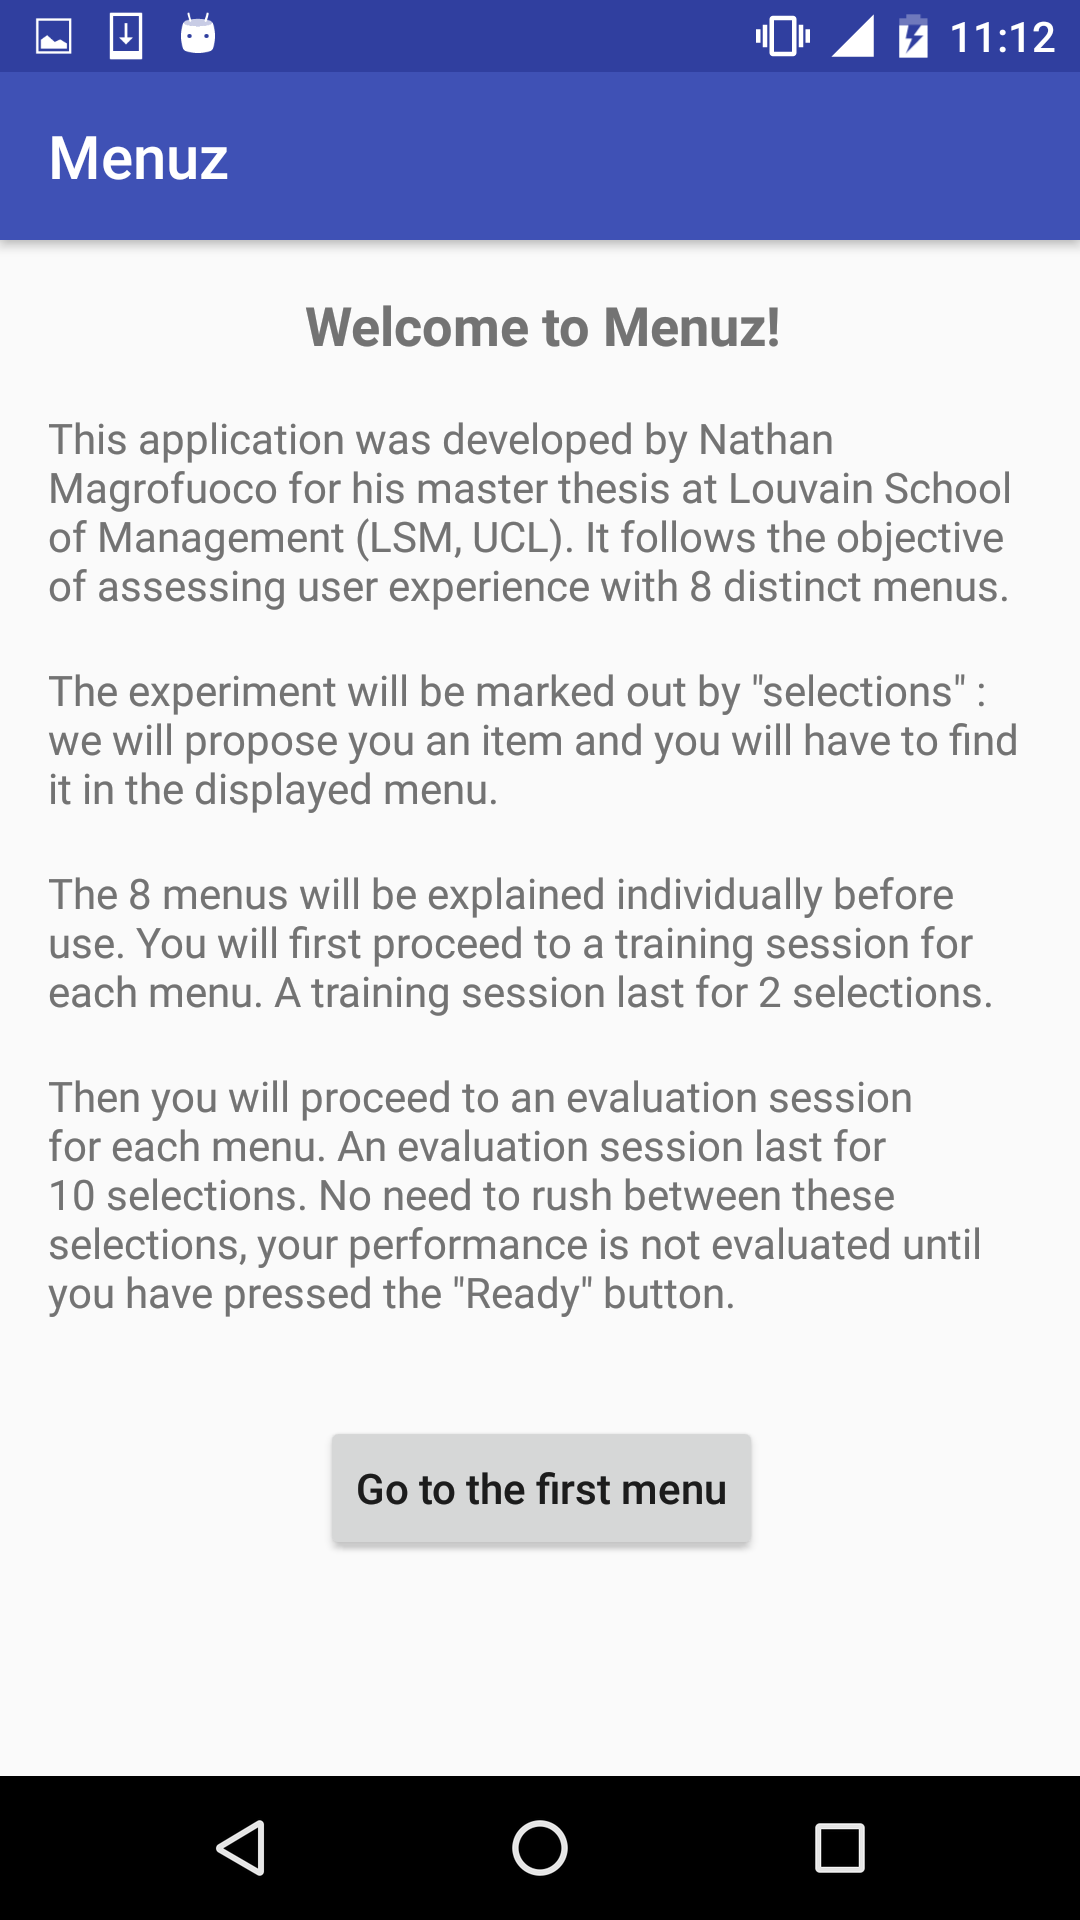
\includegraphics[scale=0.22]{img/intro_activity.png}
    \label{fig:intro_activity}
    \caption{IntroductionActivity.}
  \end{center}
\end{figure}

\newpage

\begin{figure}[!ht]
  \begin{center}
    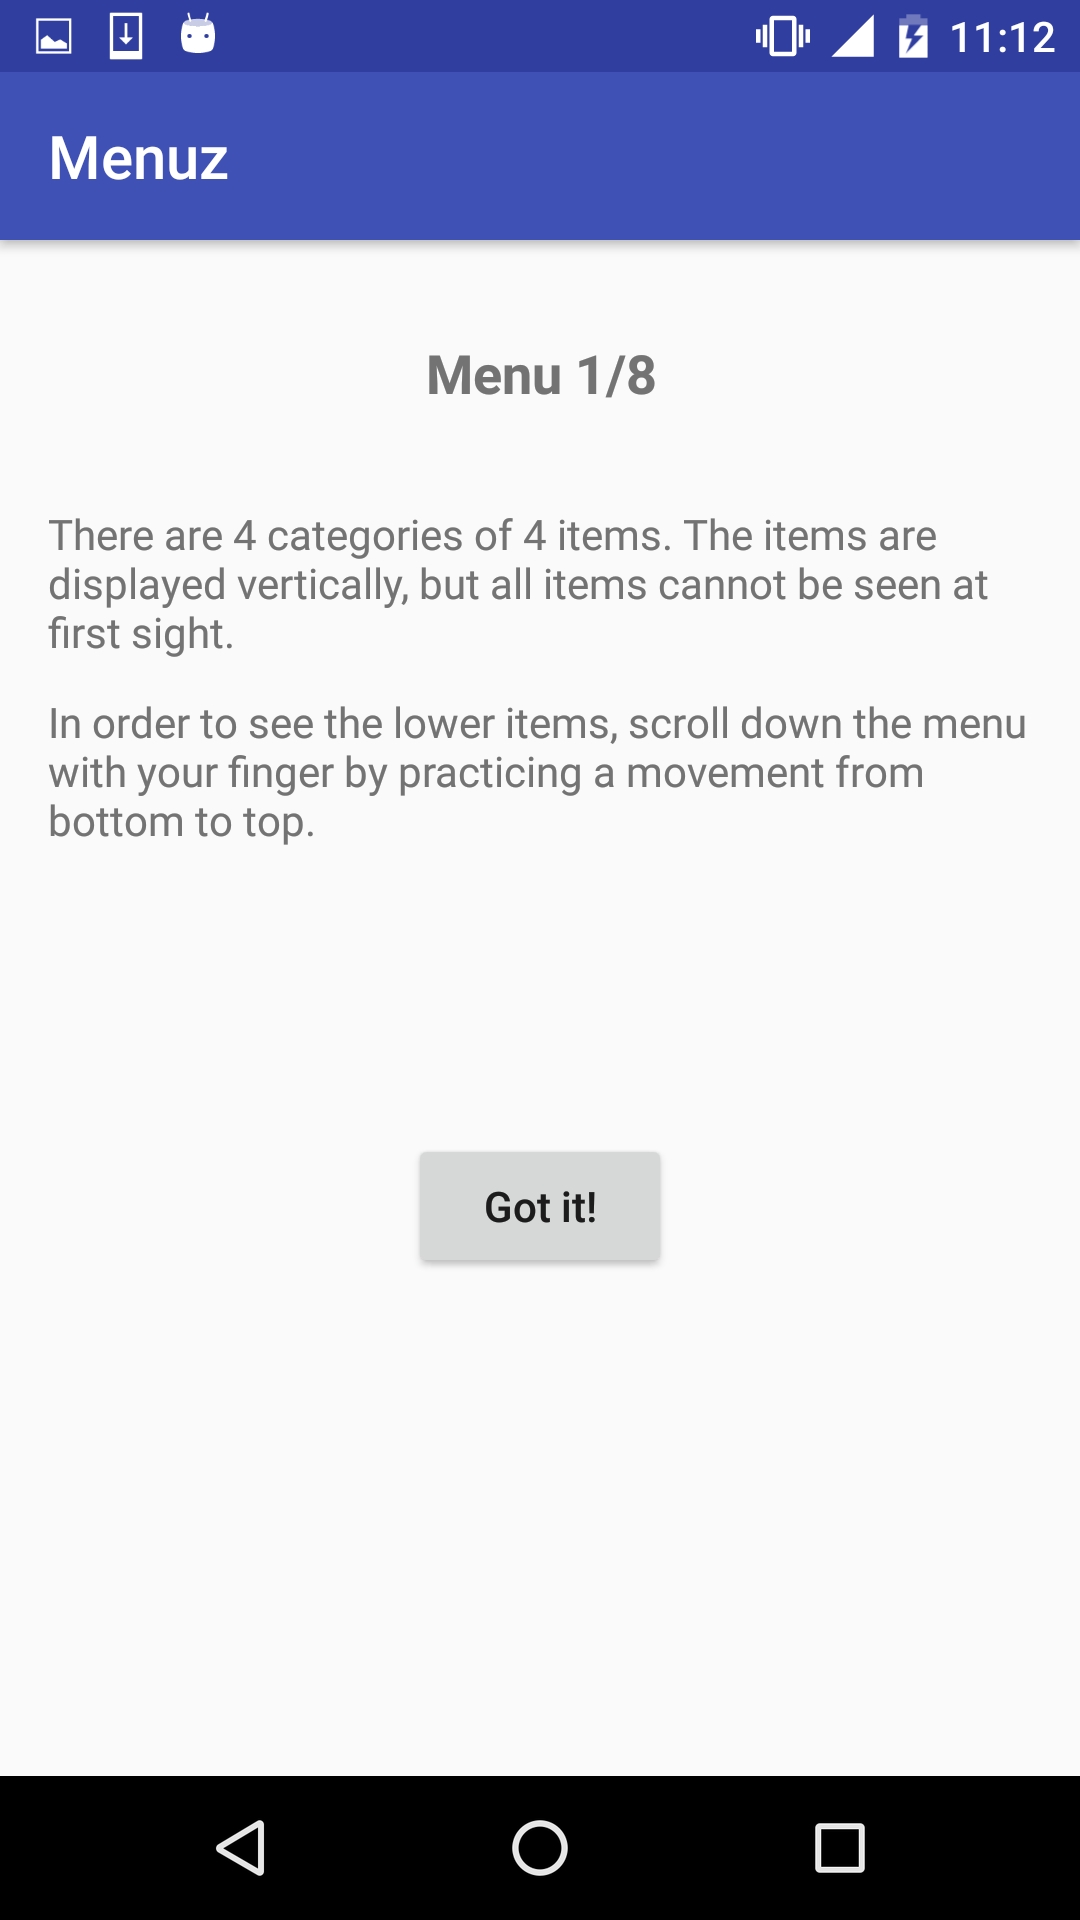
\includegraphics[scale=0.22]{img/menuintro_activity.png}
    \label{fig:menuintro_activity}
    \caption{MenuIntroductionActivity, before the 1st training session.}
  \end{center}
\end{figure}

\newpage

\begin{figure}[!ht]
  \begin{center}
    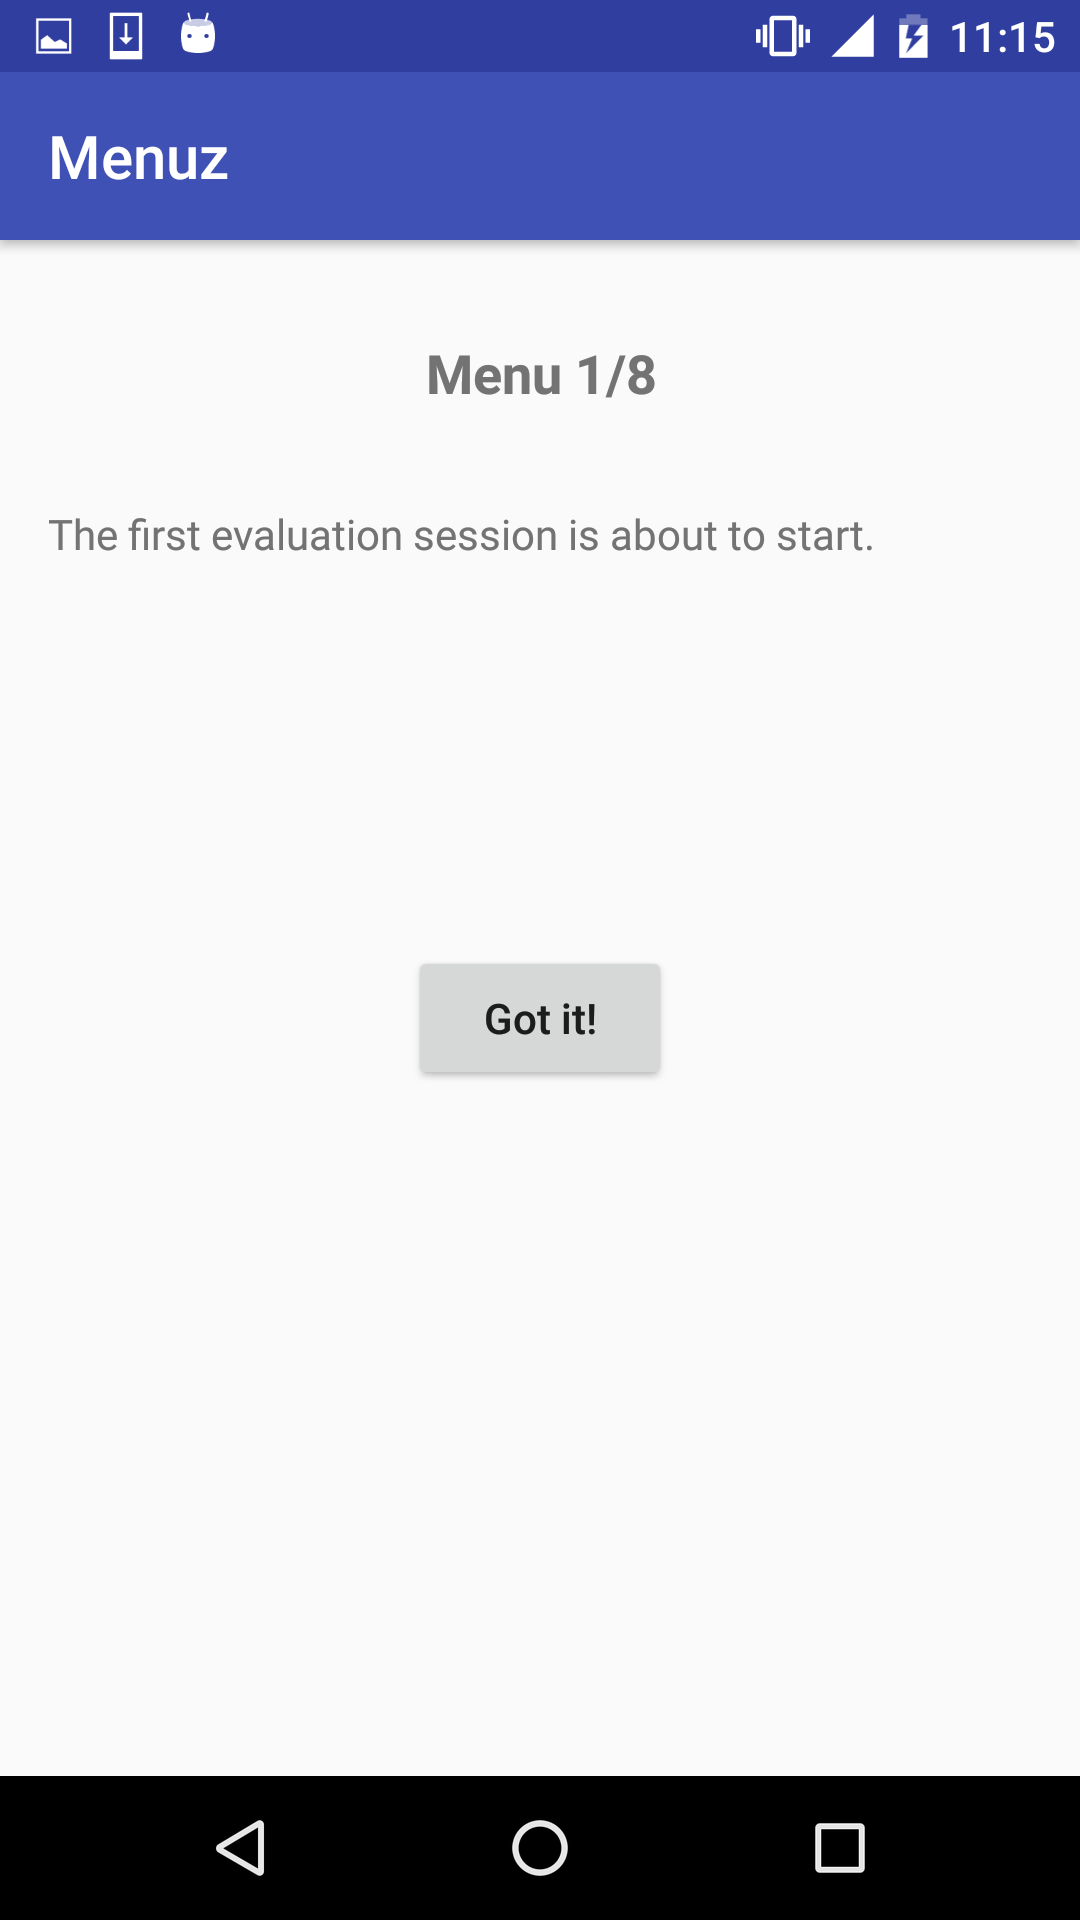
\includegraphics[scale=0.22]{img/menuintro_activityb.png}
    \label{fig:menuintro_activityb}
    \caption{MenuIntroductionActivity, before the 1st evaluation session.}
  \end{center}
\end{figure}

\newpage

\begin{figure}[!ht]
  \begin{center}
    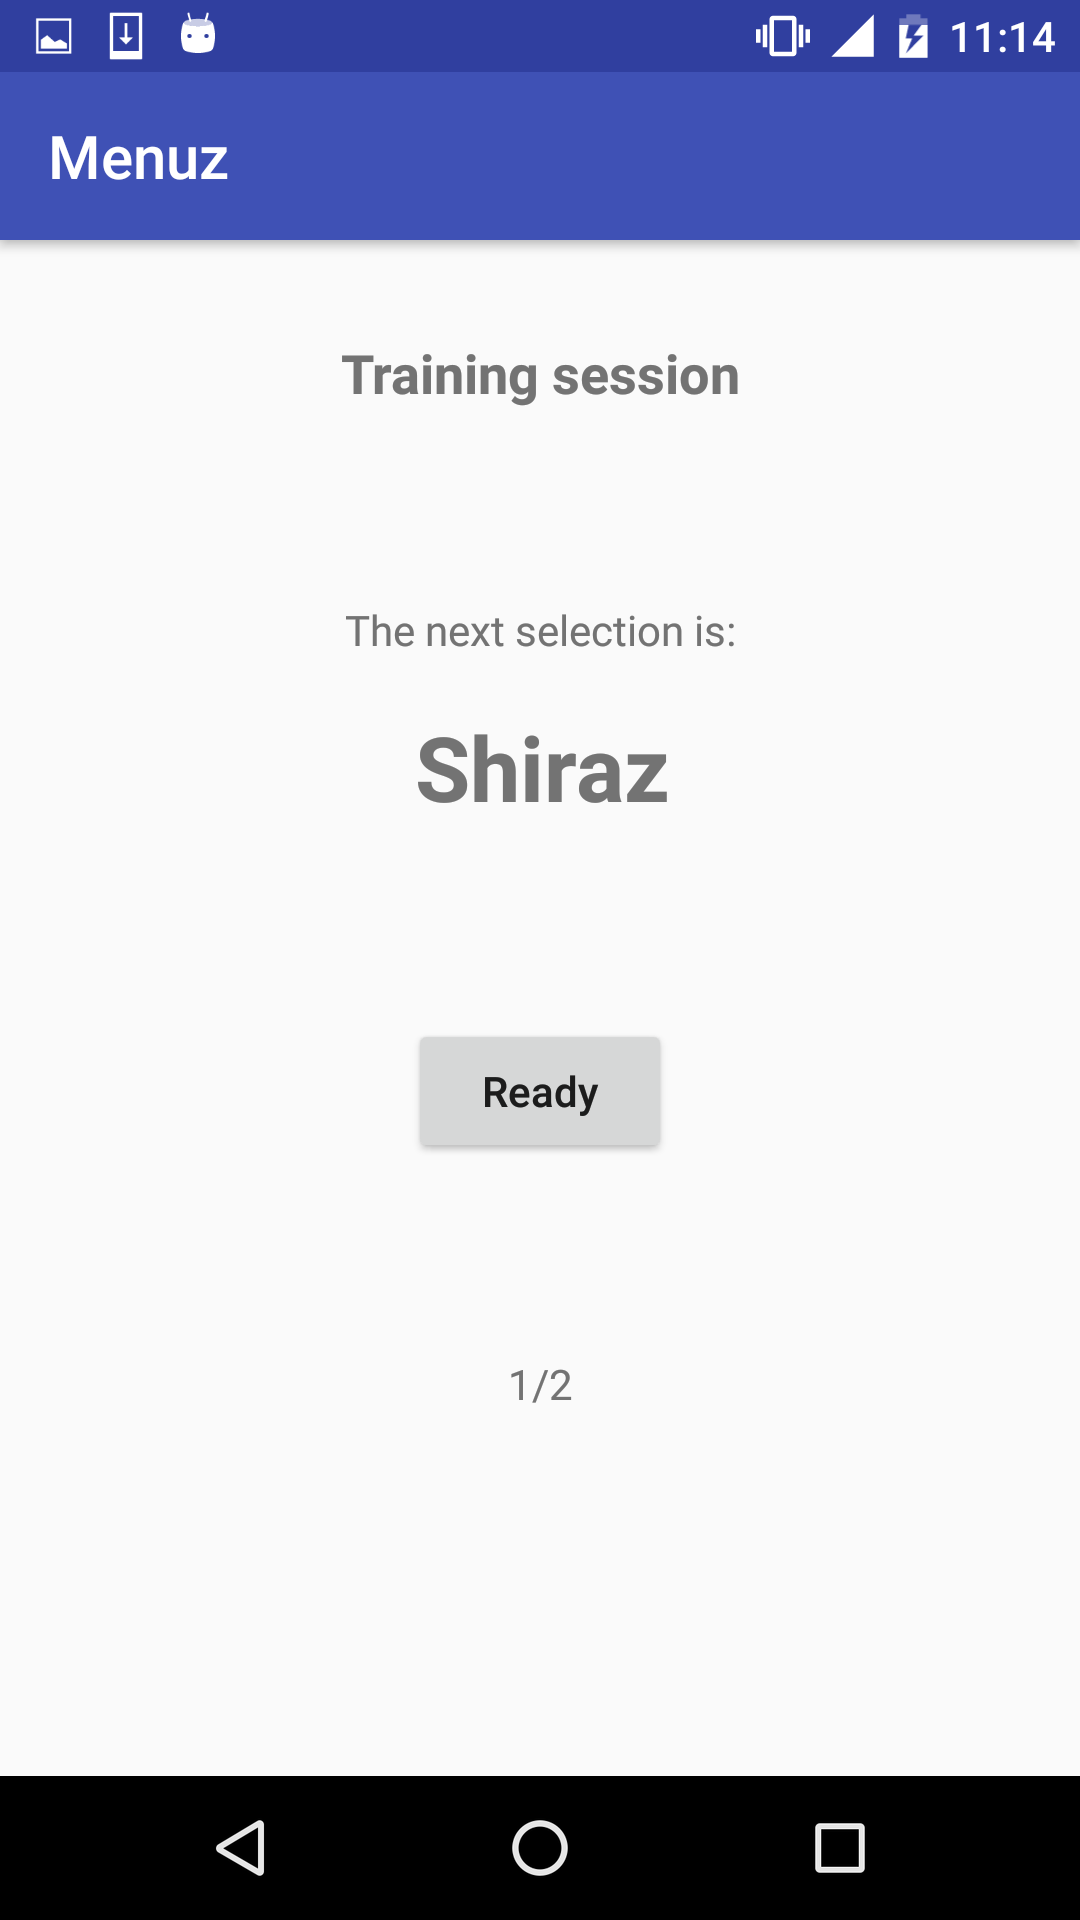
\includegraphics[scale=0.22]{img/nextselect_activity.png}
    \label{fig:nextselect_activity}
    \caption{NextSelectionActivity, during a training session.}
  \end{center}
\end{figure}

\newpage

\begin{figure}[!ht]
  \begin{center}
    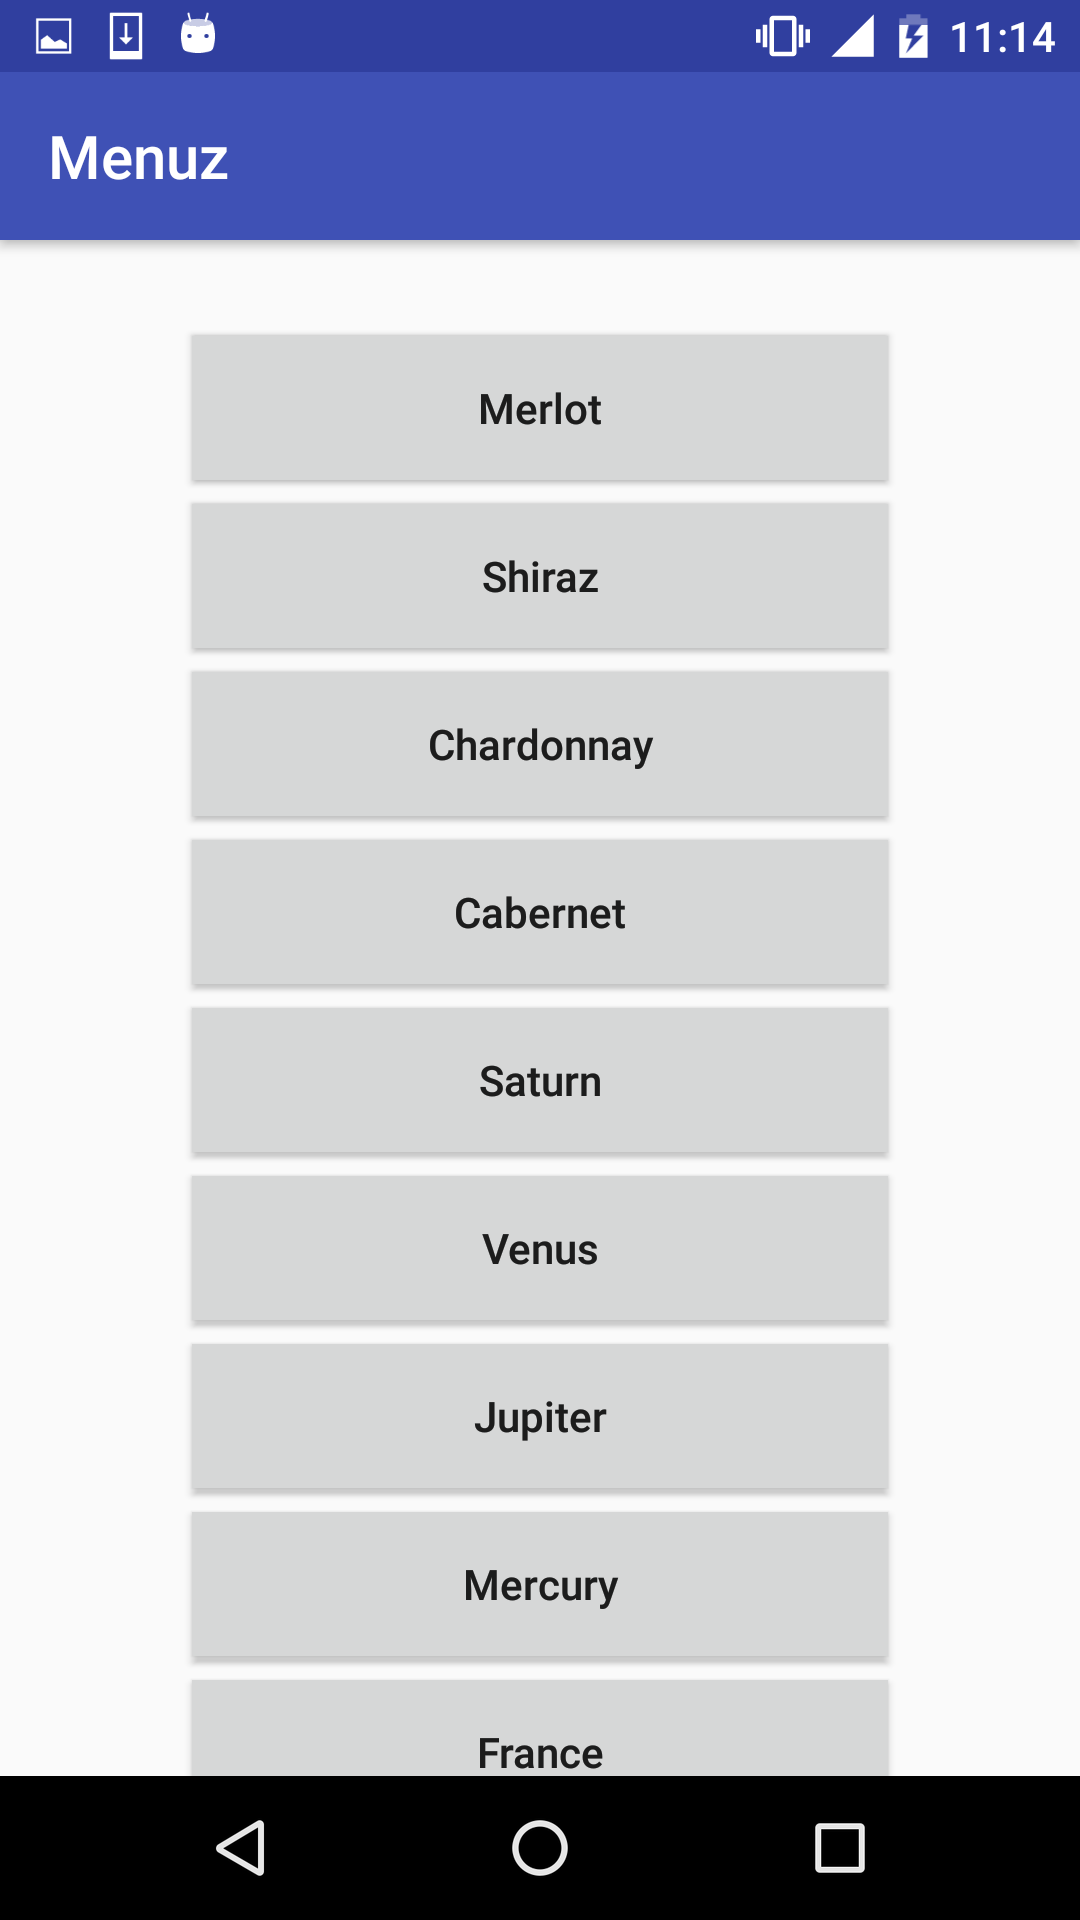
\includegraphics[scale=0.22]{img/menu.png}
    \label{fig:menu}
    \caption{MenuActivity.}
  \end{center}
\end{figure}

\newpage

\begin{figure}[!ht]
  \begin{center}
    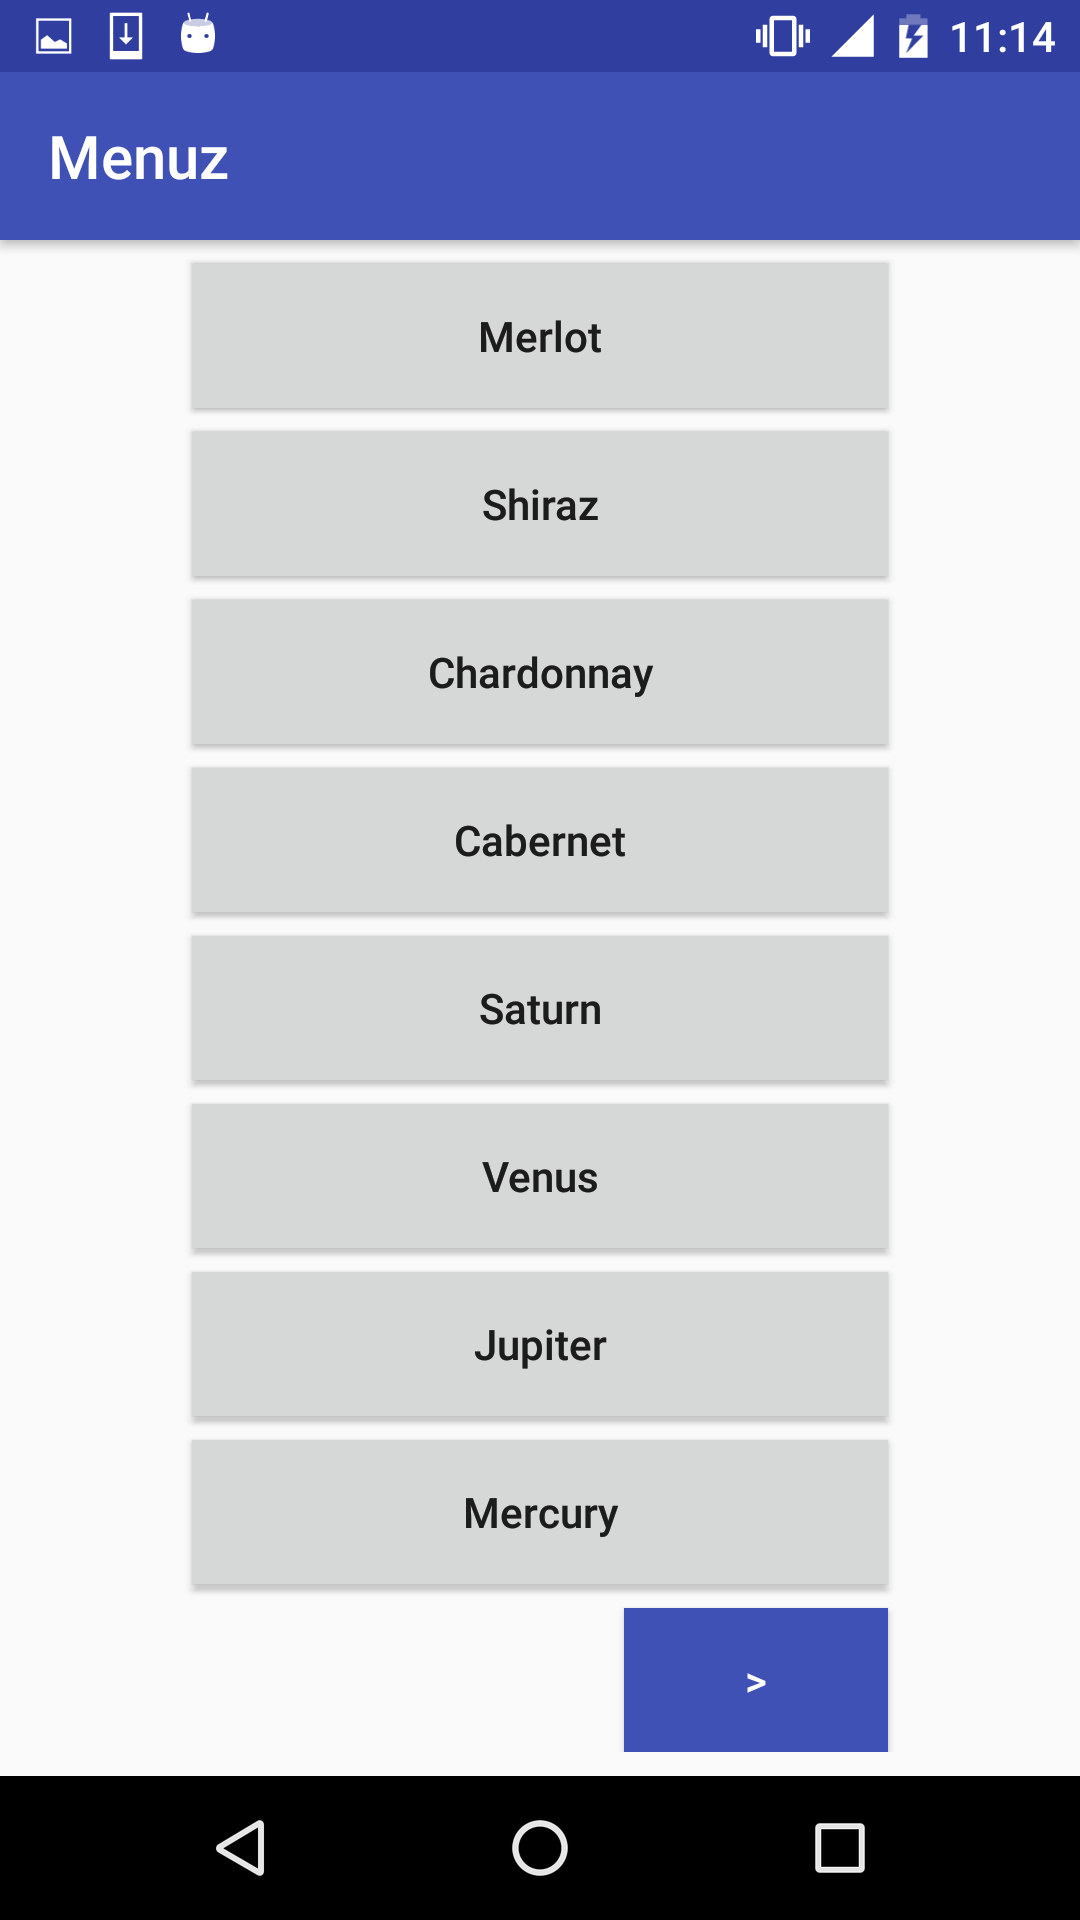
\includegraphics[scale=0.22]{img/mini_menu.png}
    \label{fig:mini_menu}
    \caption{MinimisedMenuActivity.}
  \end{center}
\end{figure}

\newpage

\begin{figure}[!ht]
  \begin{center}
    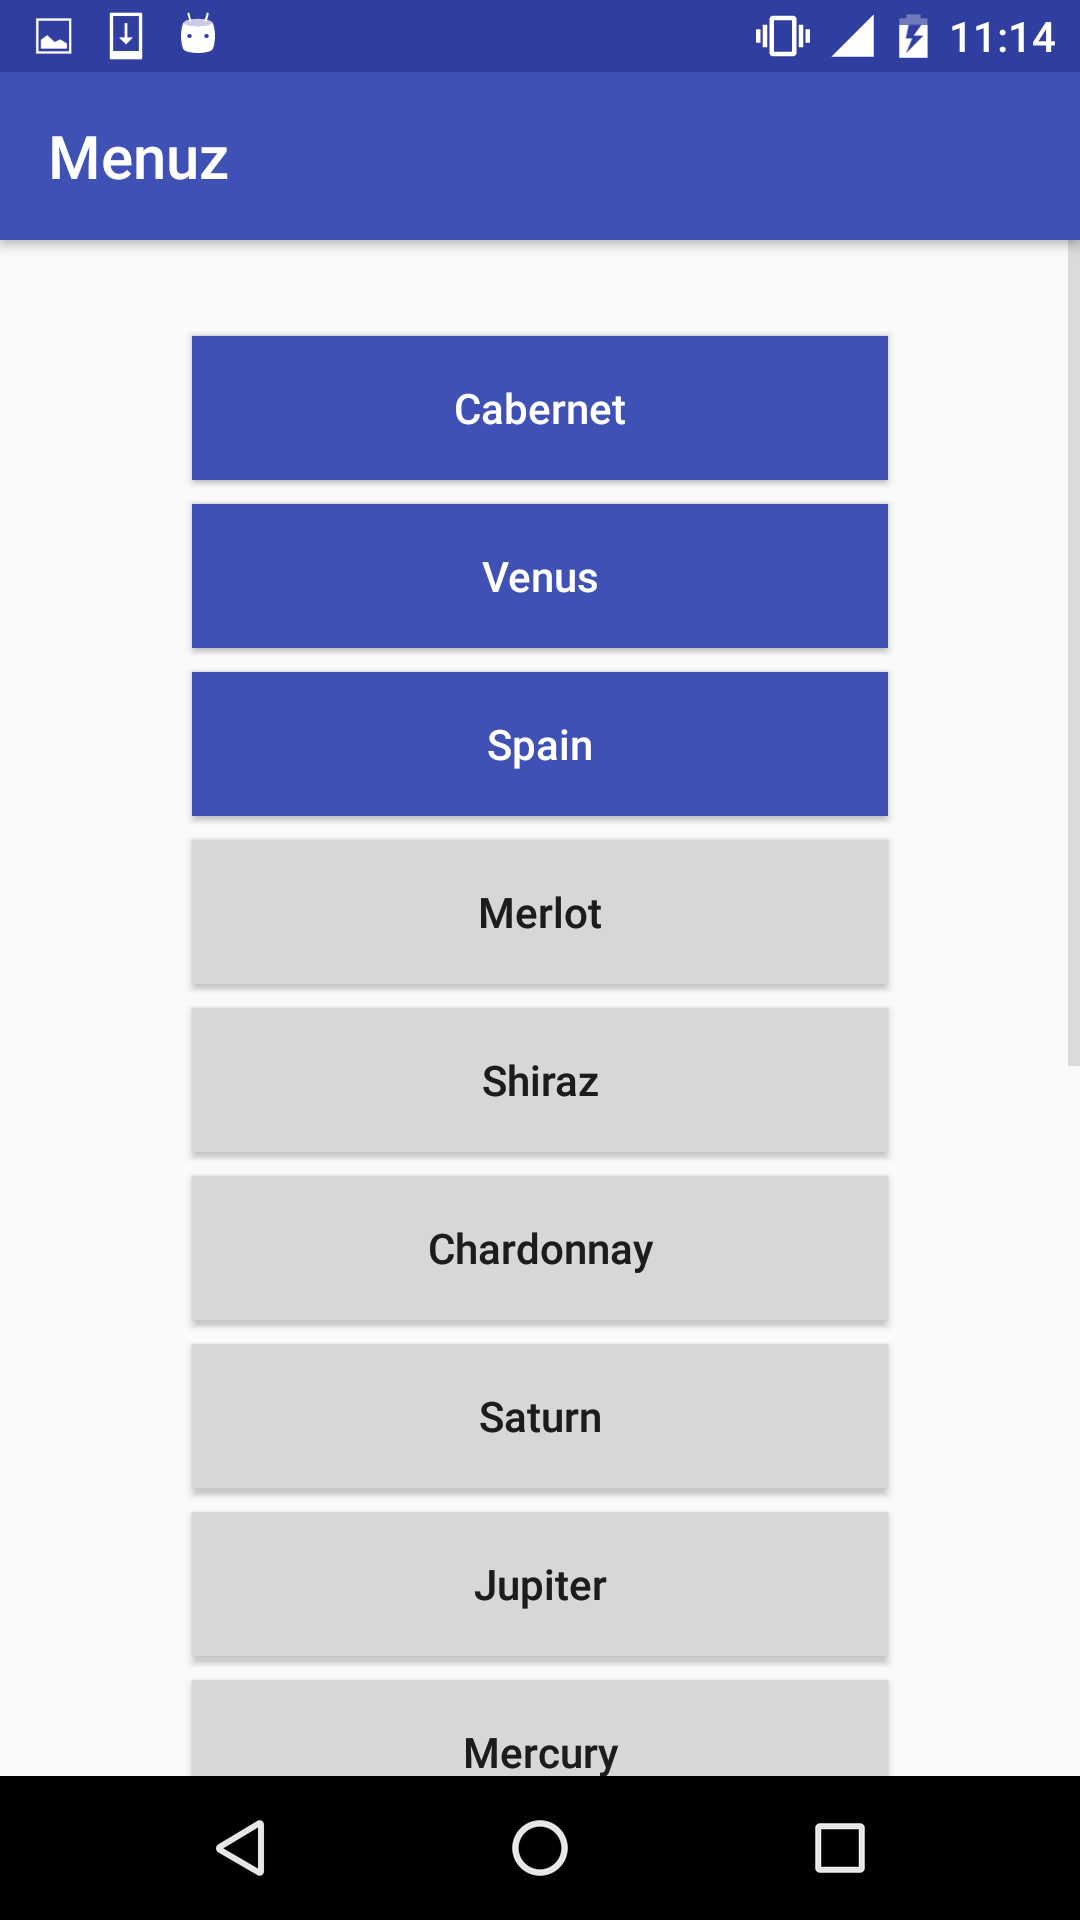
\includegraphics[scale=0.22]{img/split_menu.png}
    \label{fig:split_menu}
    \caption{SplitMenuActivity.}
  \end{center}
\end{figure}

\newpage

\begin{figure}[!ht]
  \begin{center}
    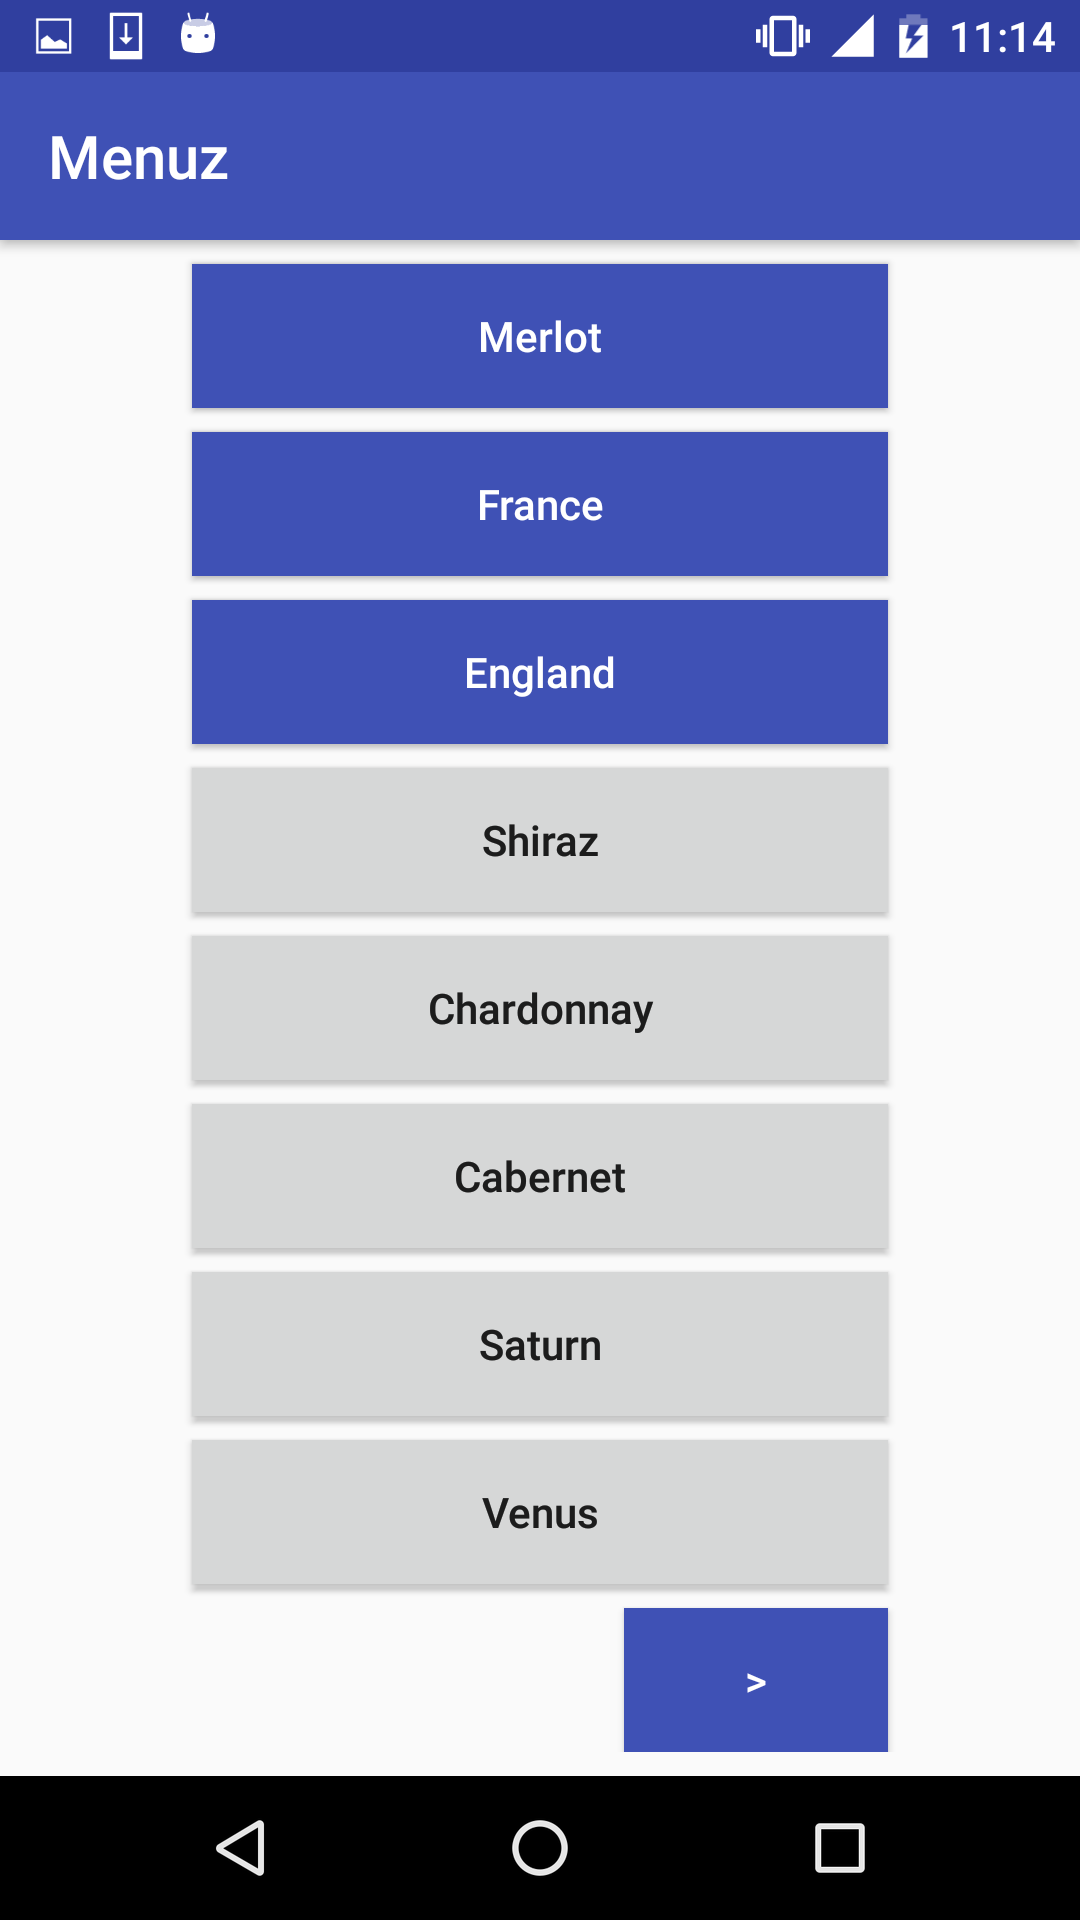
\includegraphics[scale=0.22]{img/minisplit_menu.png}
    \label{fig:minisplit_menu}
    \caption{MinimisedSplitMenuActivity.}
  \end{center}
\end{figure}

\newpage

\begin{figure}[!ht]
  \begin{center}
    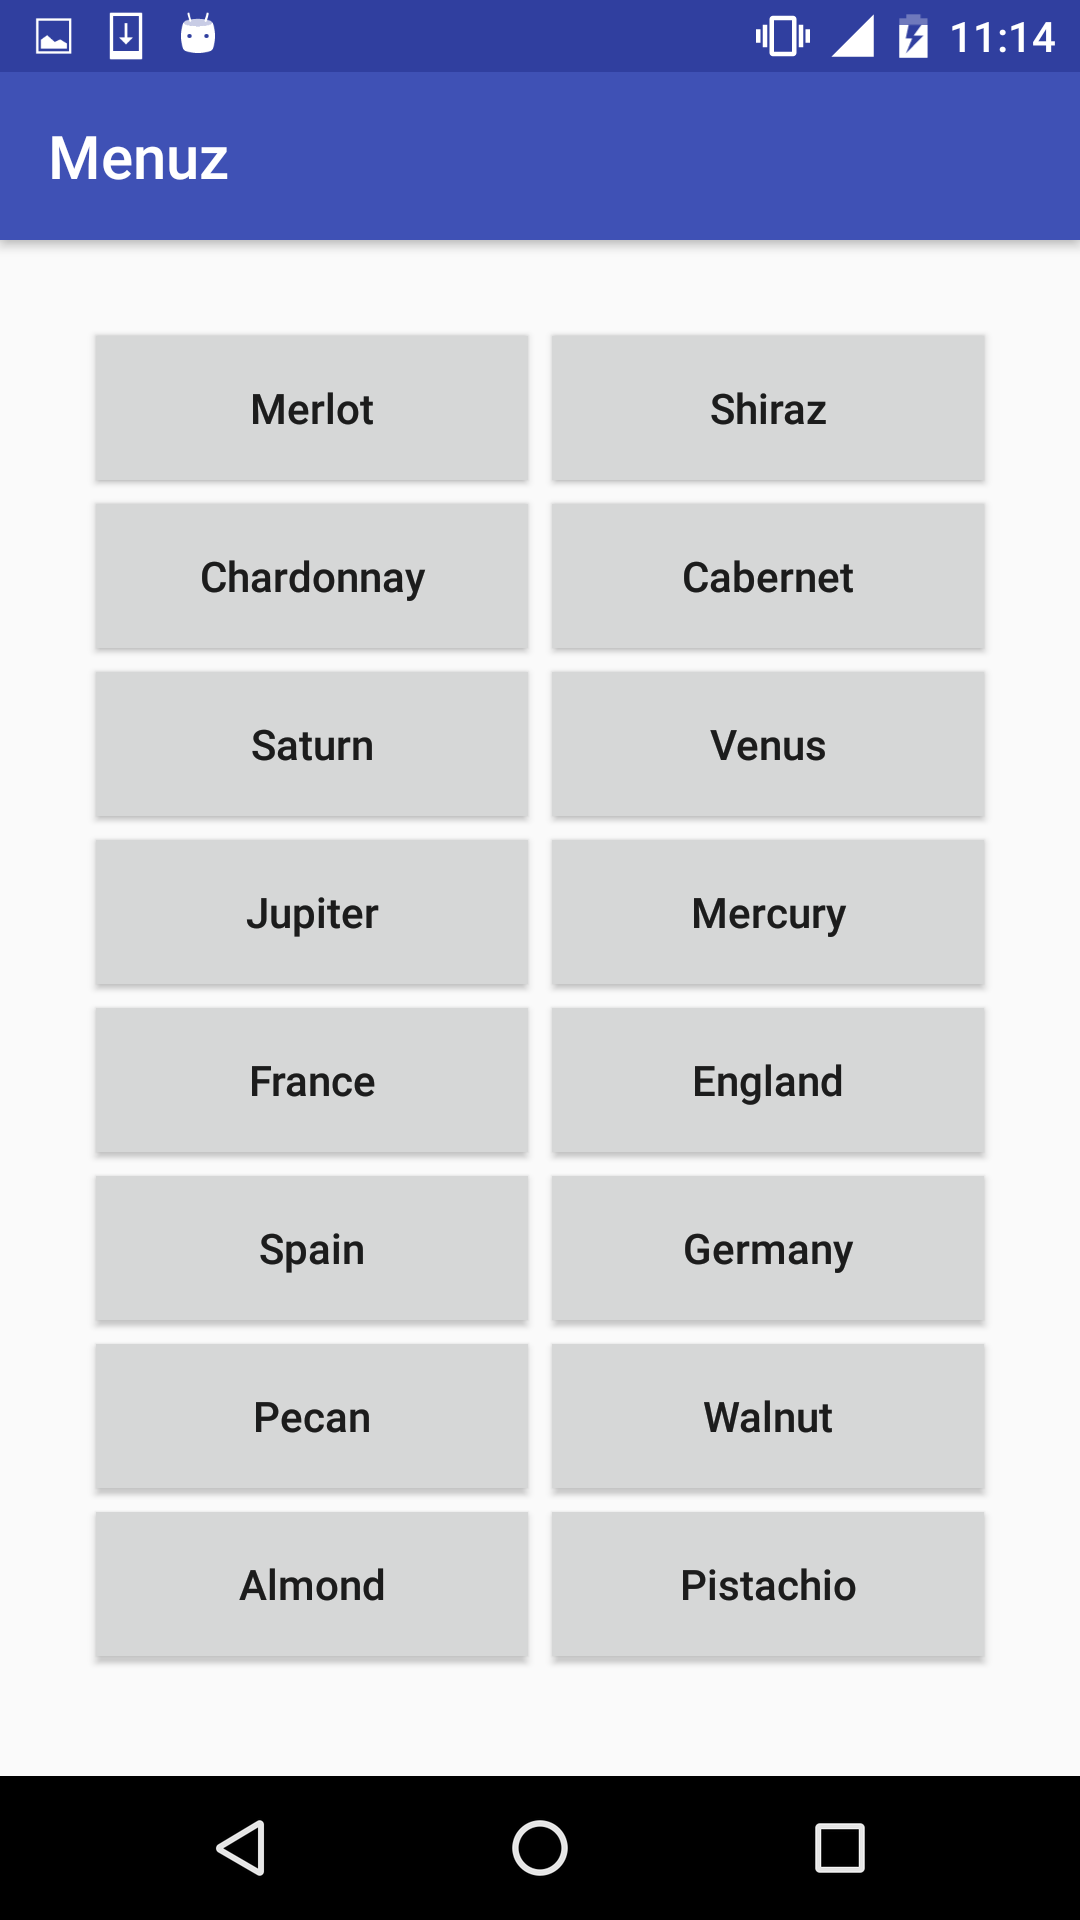
\includegraphics[scale=0.22]{img/resp_menu.png}
    \label{fig:resp_menu}
    \caption{ResponsiveMenuActivity.}
  \end{center}
\end{figure}

\newpage

\begin{figure}[!ht]
  \begin{center}
    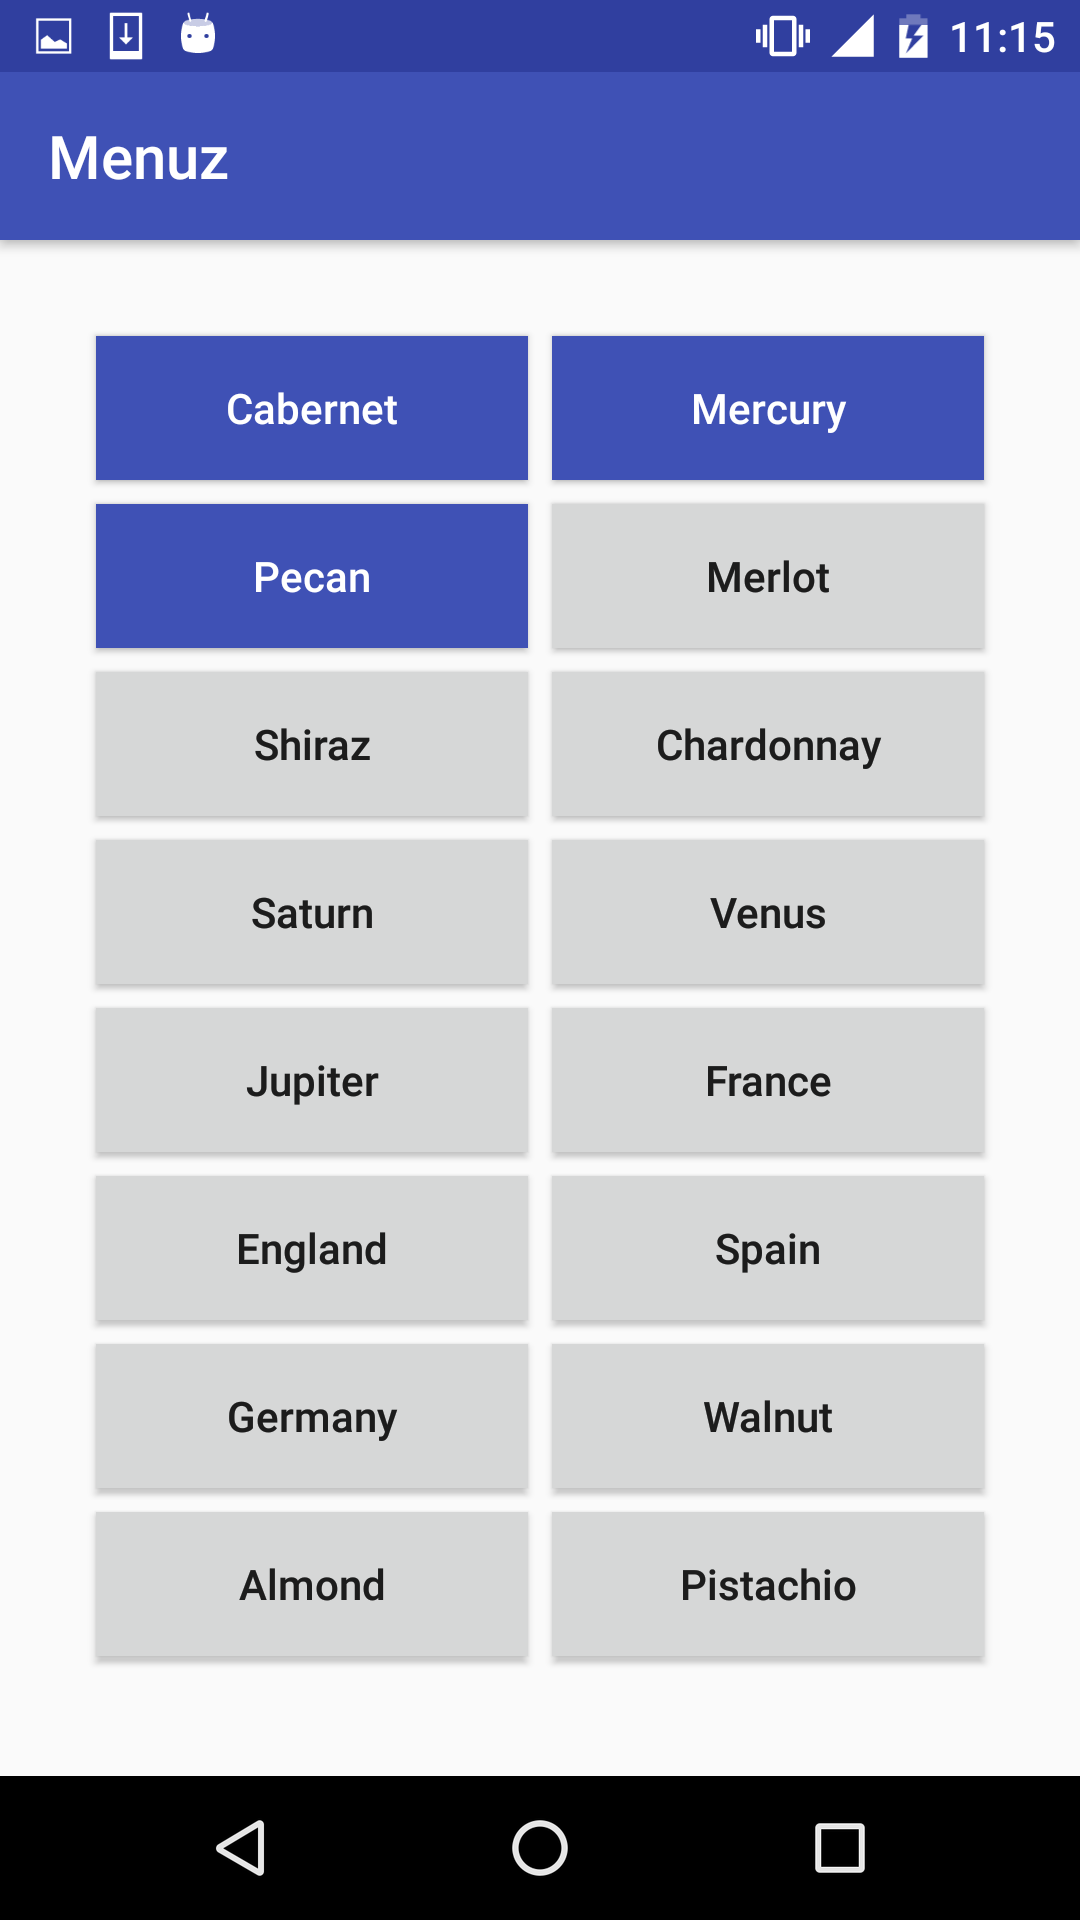
\includegraphics[scale=0.22]{img/respsplit_menu.png}
    \label{fig:respsplit_menu}
    \caption{ResponsiveSplitMenuActivity.}
  \end{center}
\end{figure}

\newpage

\begin{figure}[!ht]
  \begin{center}
    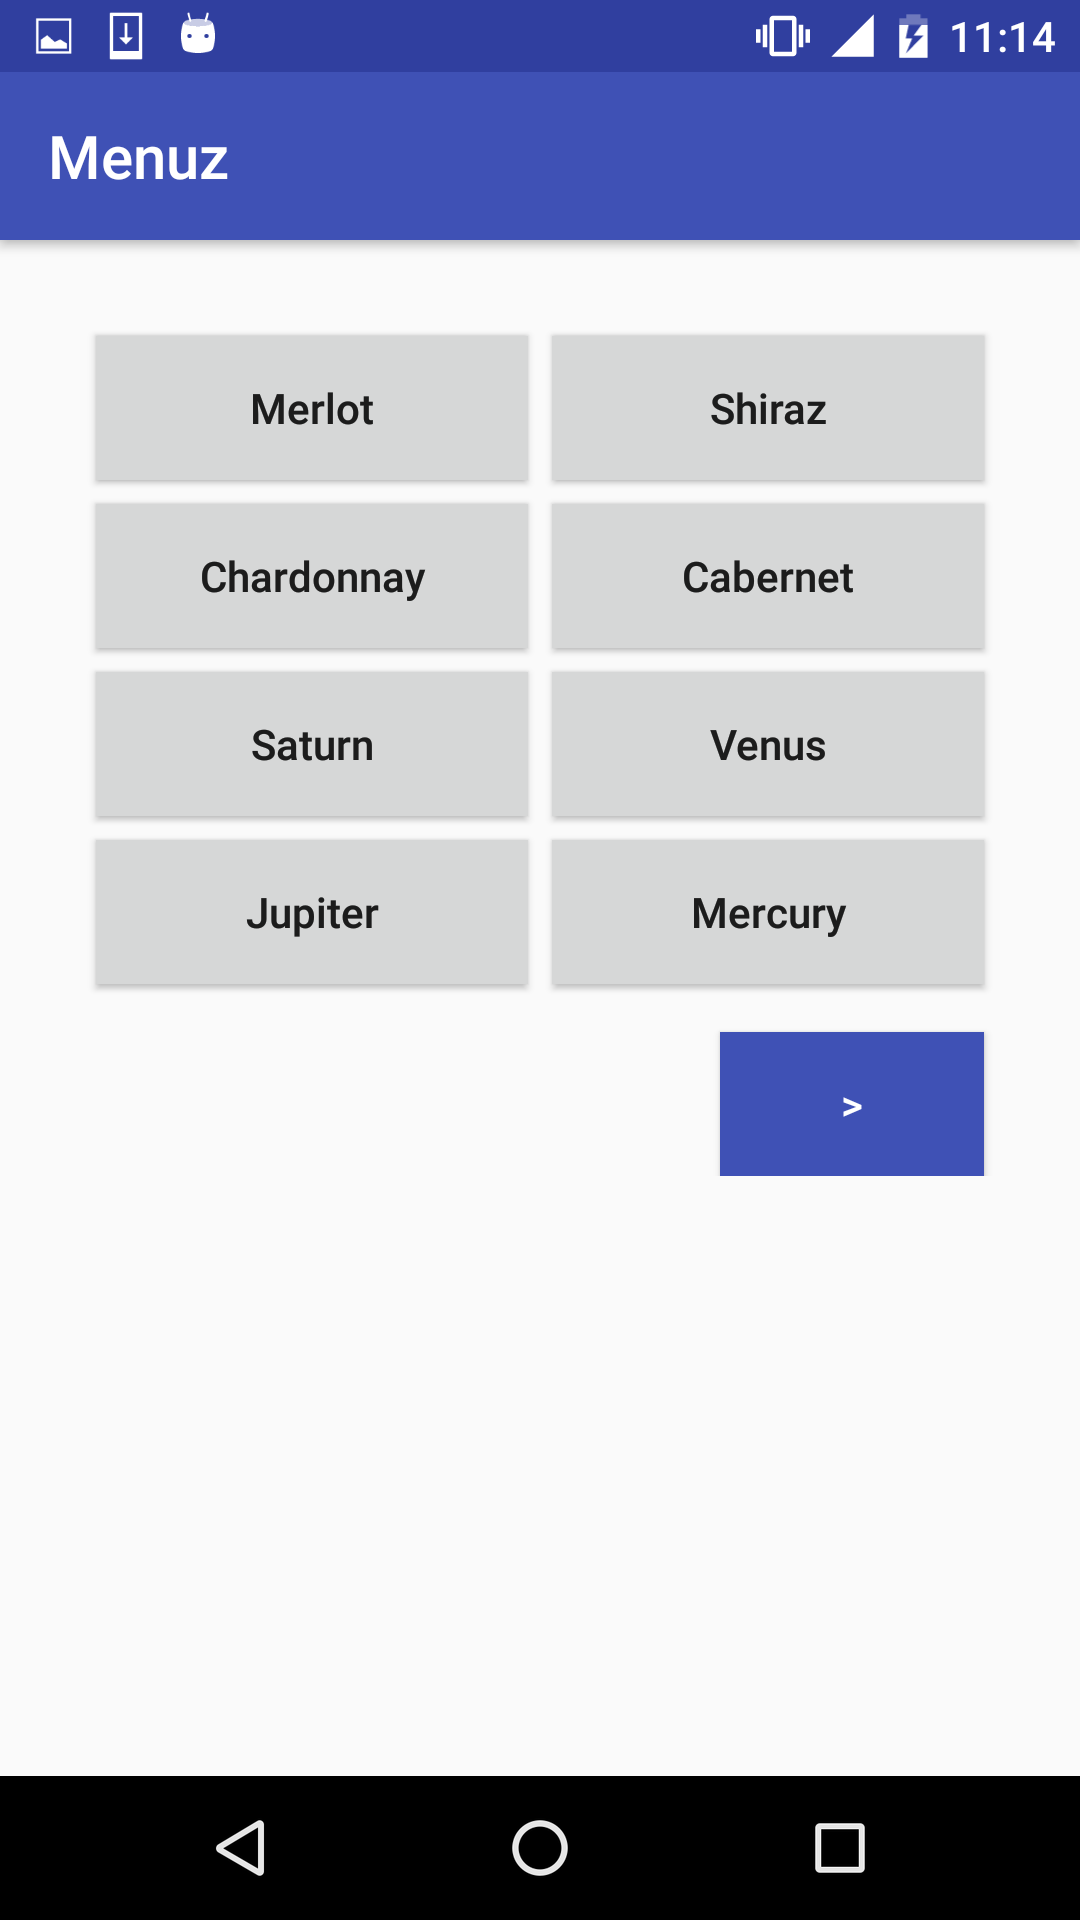
\includegraphics[scale=0.22]{img/miniresp_menu.png}
    \label{fig:miniresp_menu}
    \caption{MinimisedResponsiveMenuActivity.}
  \end{center}
\end{figure}

\newpage

\begin{figure}[!ht]
  \begin{center}
    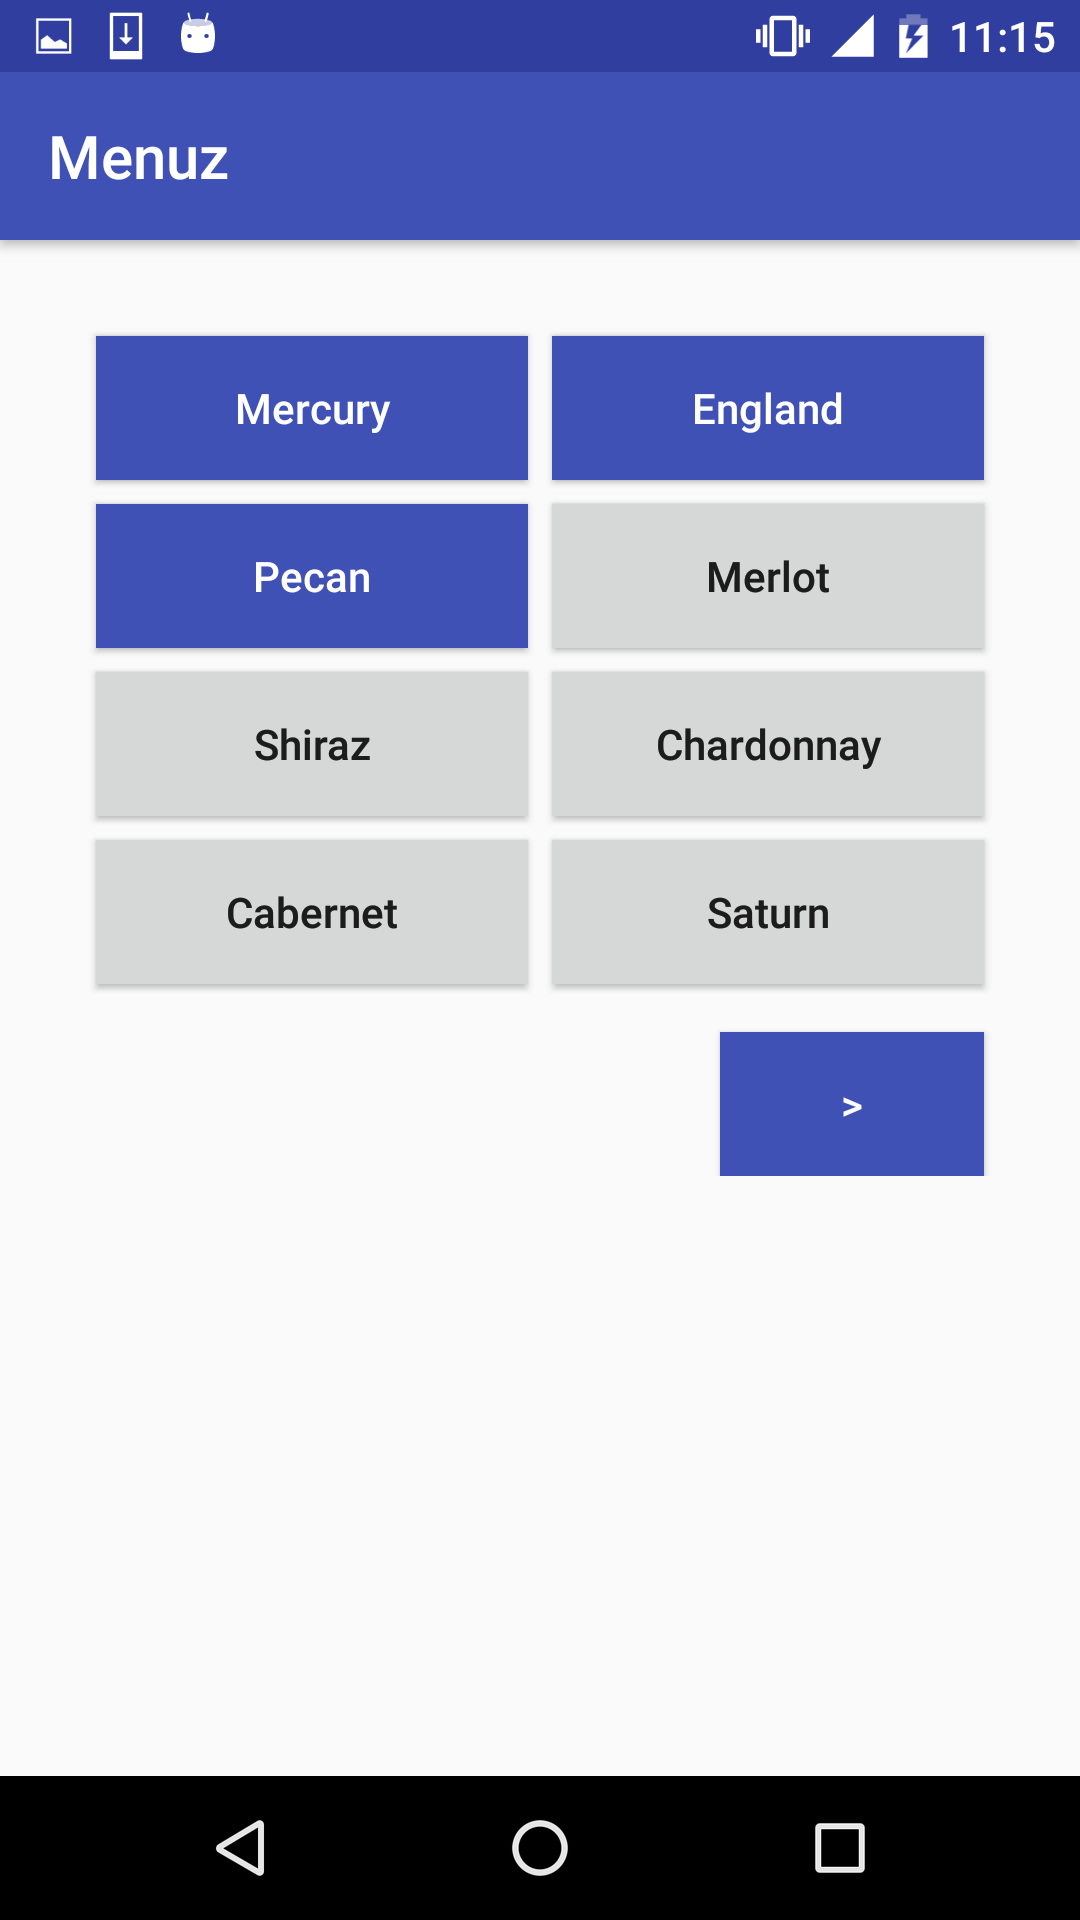
\includegraphics[scale=0.22]{img/minirespsplit_menu.png}
    \label{fig:minirespsplit_menu}
    \caption{MinimisedResponsiveSplitMenuActivity.}
  \end{center}
\end{figure}

\newpage

\begin{figure}[!ht]
  \begin{center}
    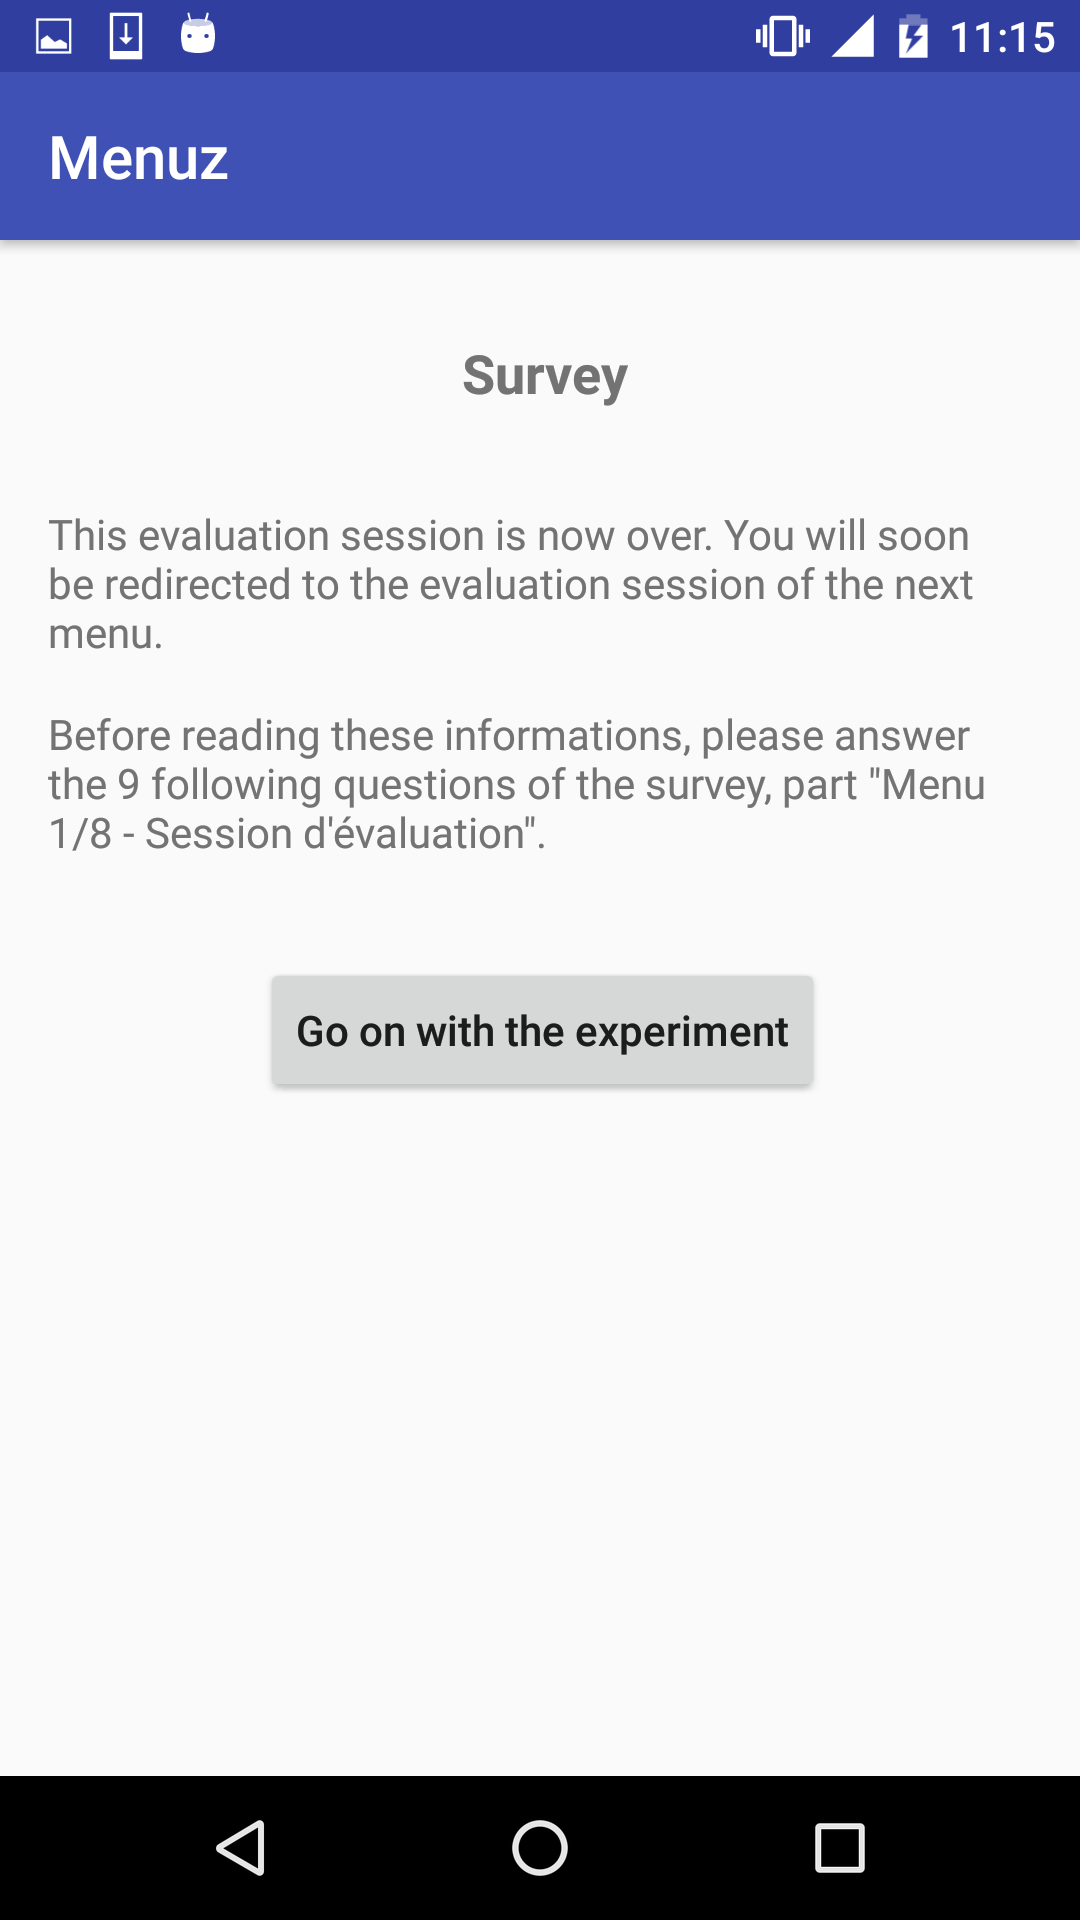
\includegraphics[scale=0.22]{img/survey_activity.png}
    \label{fig:survey_activity}
    \caption{SurveyActivity, at the end of the 1st evaluation session.}
  \end{center}
\end{figure}

\newpage

\begin{figure}[!ht]
  \begin{center}
    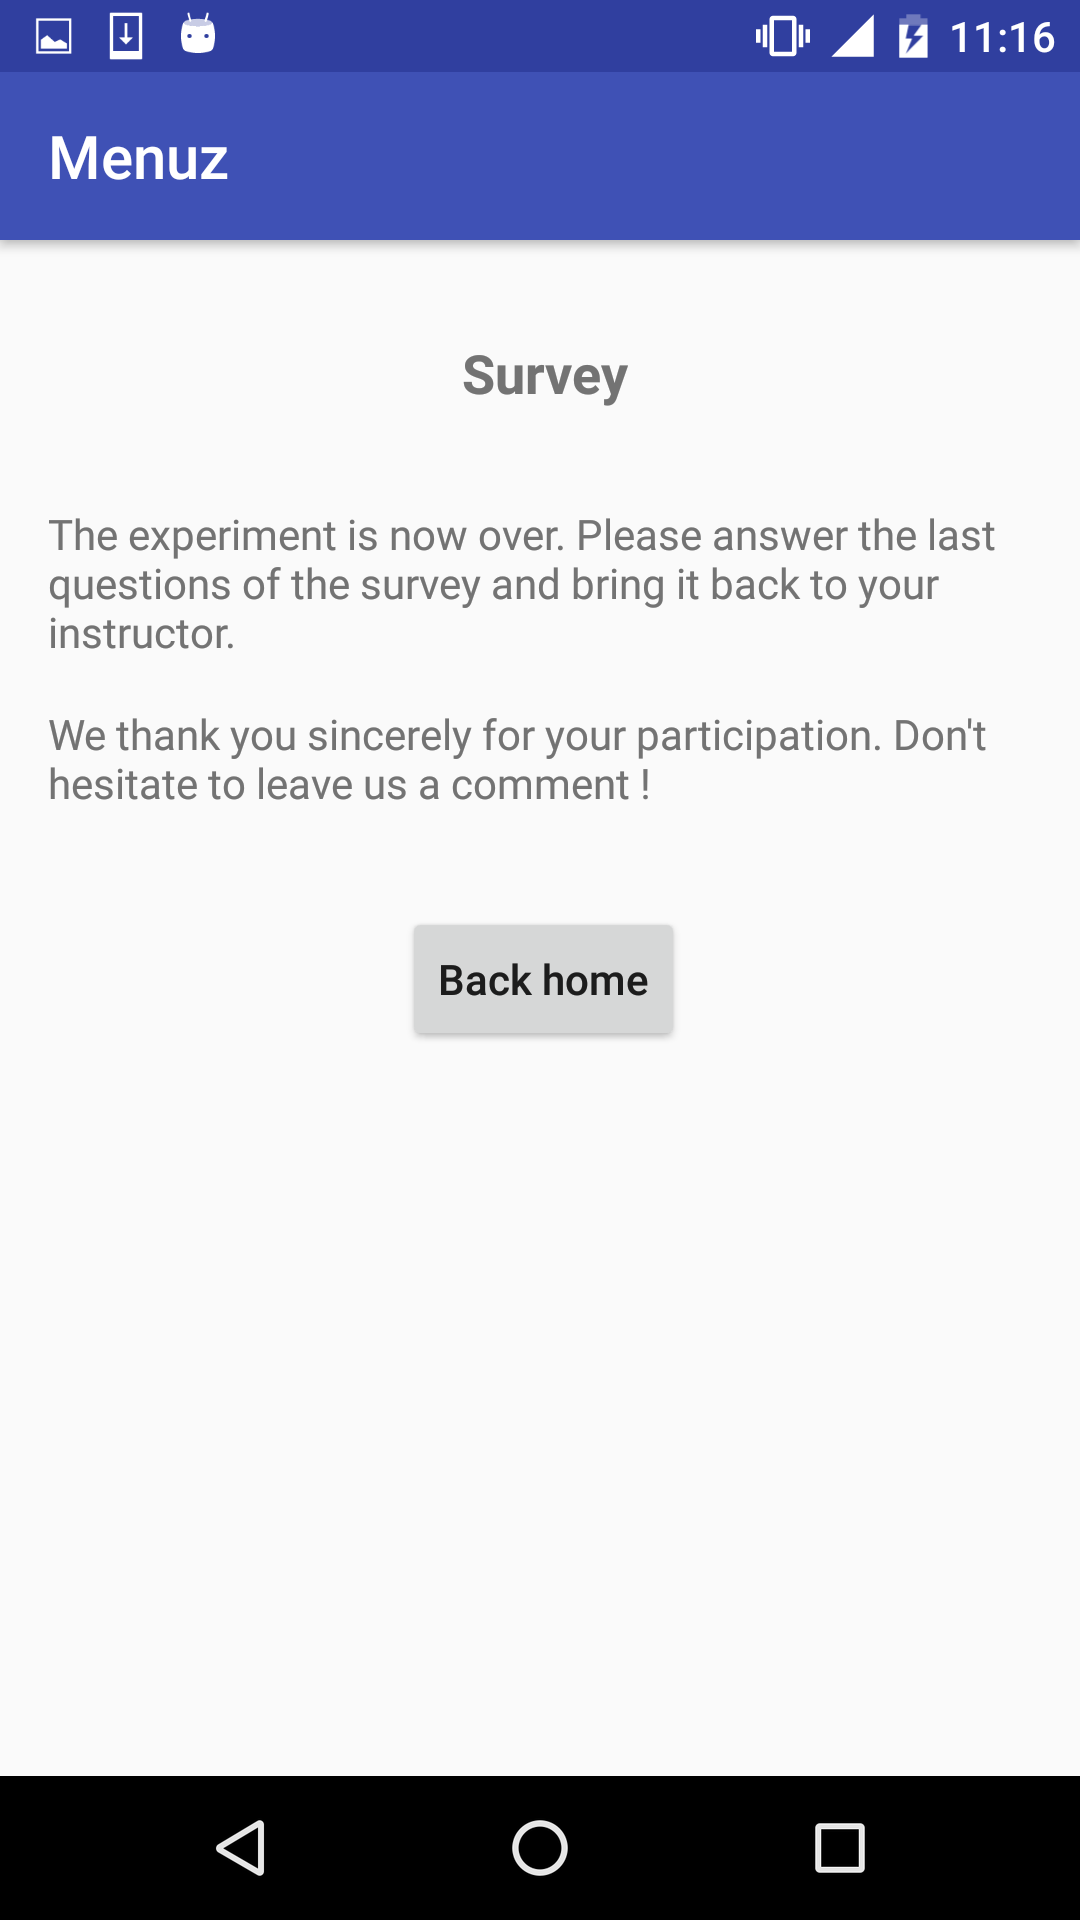
\includegraphics[scale=0.22]{img/survey_activityb.png}
    \label{fig:survey_activityb}
    \caption{SurveyActivity, at the end of the experiment.}
  \end{center}
\end{figure}

\newpage

\chapter{Get the app (How to)}
The Android application developed during the experiment is available as an open 
source repository on GitHub, see github.com/nmagrofuoco/menuz. The 
application is currently implemented in its French version. A readme file is 
available to switch the application to its English version. The repository also 
stores the sources of the dissertation.